\DefineShortVerb{\!}
\chapter{Απόδοση}
\section{Μεθοδολογία μέτρησης απόδοσης}
\label{chapter:bench_method}
\noindent
Η μέτρηση των επιδόσεων την υλοποίησης σε GPU πραγματοποιήθηκε με την βοήθεια μιας τροποποιημένης εκδοχής του υπάρχοντος συστήματος \begin{english}benchmarking\end{english} της δημοσίευσης \cite{PlatisTheoharis03}, το οποίο είναι διαθέσιμο στον χρήστη μέσω του εκτελέσιμου \verb!Bench!. Στο σύστημα αυτό έχουν προστεθεί οι αλγόριθμοι που εκτελούνται στην GPU.

Η μέθοδος χρονομέτρησης των αλγορίθμων σε \begin{english}GPU\end{english} διαφέρει από αυτήν που χρησιμοποιείται στους ακολουθιακούς αλγόριθμους. Στους ακολουθιακούς αλγόριθμους τα δεδομένα εισόδου είναι αποθηκευμένα στην κύρια μνήμη του συστήματος \begin{english}(RAM)\end{english} πριν την εκτέλεση του αλγορίθμου. Έτσι, ο χρόνος που καταγράφεται κατά την εκτέλεση του \begin{english}\verb!Bench!\end{english} είναι ο καθαρός χρόνος επεξεργασίας των δεδομένων. Αντίθετα, στην επεξεργασία σε \begin{english}GPU\end{english}, η εκτέλεση ενός αλγορίθμου  περιλαμβάνει την μεταφορά των δεδομένων από την κύρια μνήμη του συστήματος στην μνήμη της \begin{english}GPU\end{english}, την επεξεργασία τους και την μεταφορά των αποτελεσμάτων πίσω στην κύρια μνήμη. Οι χρόνοι των μεταφορών από και προς την \begin{english}GPU\end{english} αποτελούν σημαντικό παράγοντα του συνολικού χρόνου εκτέλεσης των αλγορίθμων σε \begin{english}GPU\end{english}. Επίσης, η ταχύτητα των μεταφορών αυτών μπορεί να διαφέρει σημαντικά ανάμεσα σε 
διαφορετικά μοντέλα \begin{english}GPU\end{english} λόγω διαφορετικής αξιοποίησης του διαύλου \begin{english}PCI Express\end{english}. Για τους λόγους αυτούς, και για την δυνατότητα αμεσότερης σύγκρισης της υπολογιστικής απόδοσης μεταξύ \begin{english}GPU\end{english} και \begin{english}CPU\end{english}, οι χρόνοι μεταφοράς από και προς την \begin{english}GPU\end{english} καταγράφονται ξεχωριστά από τον καθαρό χρόνο επεξεργασίας. Ο χρόνος μεταφοράς προς την \begin{english}GPU\end{english} αντιστοιχεί στην εγγραφή των δεδομένων στα \begin{english}buffer\end{english} εισόδου και αναφέρεται ως \textit{χρόνος εγγραφής}. Η αντίθετη μεταφορά αντιστοιχεί στην ανάγνωση των \begin{english}buffer\end{english} εξόδου και ονομάζεται \textit{χρόνος ανάγνωσης}. 

Οι μετρήσεις των χρόνων εγγραφής και ανάγνωσης διαφέρουν από αυτές των χρόνων επεξεργασίας. Όπως θα αναλυθεί στην συνέχεια του κειμένου, η κάθε χρονομέτρηση περιλαμβάνει μερικές επαναλήψεις της εκτέλεσης του αλγορίθμου που ελέγχεται. Ο χρόνος επεξεργασίας που μετράται είναι το άθροισμα των χρόνων επεξεργασίας κάθε επανάληψης. Αντίθετα, οι χρόνοι εγγραφής και ανάγνωσης αντιστοιχούν στον χρόνο που απαιτείται για την μεταφορά δεδομένων προς ή από την GPU μία φορά.   

\subsubsection*{Συστήματα Δοκιμών}

Οι μετρήσεις επιδόσεων των διάφορων υλοποιήσεων των αλγορίθμων έγιναν σε τρία διαφορετικές συνθέσεις υπολογιστών. Αυτό έγινε για την εξασφάλιση μιας πληρέστερης εικόνας σχετικά με την επίδραση του υλικού στις επιδόσεις αυτές, με ιδιαίτερη έμφαση στην διαφορά των επιδόσεων ανάμεσα σε διαφορετικές γενιές GPU. Τα συστήματα που χρησιμοποιήθηκαν είχαν τις εξής προδιαγραφές:

\begin{description}
  \item[Σύστημα 1:]\textbf{CPU:}Intel Core i7 920 με συχνότητα 2,67 GHz \textbf{GPU:} Nvidia GTX285 %melissa
  \item[Σύστημα 2:]\textbf{CPU:}Intel Core i7 2600 με συχνότητα 3,4 GHz \textbf{GPU:} Nvidia GTX560 %melissa2
  \item[Σύστημα 3:]\textbf{CPU:}AMD Phenom II 1055T με συχνότητα 2,8 GHz \textbf{GPU:} Nvidia GTX560Ti %Js1
\end{description}

Στα πρώτα δύο συστήματα οι μετρήσεις έγιναν σε λειτουργικό σύστημα Linux. Στο σύστημα 3 έγιναν σε Linux και Windows 7. Τα αποτελέσματα των μετρήσεων στα δύο λειτουργικά συστήματα παρουσιάζονται χωριστά.

\subsubsection*{Ρυθμίσεις Δοκιμών}

Οι μετρήσεις έγιναν μέσω του \begin{english}\verb!fullbench.sh!\end{english}. Σε όλες τις περιπτώσεις χρησιμοποιήθηκε βήμα ποσοστού τεμνόμενων ζευγών 10\%. Έγιναν δύο σειρές δοκιμών. Η πρώτη σειρά περιείχε συνολικά 25 εκατομμύρια ελέγχους τομής στις εξής διαρρυθμίσεις:

\begin{enumerate*}
\item 2.5 εκατομμύρια ζεύγη/10 επαναλήψεις
\item 250 χιλιάδες ζεύγη/100 επαναλήψεις 
\item 25 χιλιάδες ζεύγη/1000 επαναλήψεις  
\end{enumerate*}

Η δεύτερη σειρά περιείχε 50 εκατομμύρια ελέγχους στις εξής διαρρυθμίσεις:

\begin{enumerate*}
\item 5 εκατομμύρια ζεύγη/10 επαναλήψεις
\item 500 χιλιάδες ζεύγη/100 επαναλήψεις 
\item 50 χιλιάδες ζεύγη/1000 επαναλήψεις   
\end{enumerate*}

\section{Αποτελέσματα}
\label{chapter:bench_interpret}
\noindent Η ενότητα αυτή παρουσιάζει τα συμπεράσματα τα οποία προέκυψαν από τα αποτελέσματα των μετρήσεων σε τέσσερα διακριτά θέματα:
\begin{enumerate}
\item Την σύγκριση επιδόσεων μεταξύ των υλοποιήσεων σε CPU και GPU.
\item Την αποτελεσματικότητα των διάφορων μορφών αλγορίθμων σε CPU και GPU.
\item Την επίδραση των ρυθμίσεων δοκιμών στα αποτελέσματα.
\item Την σύγκριση επιδόσεων μεταξύ λειτουργικών συστημάτων.
\end{enumerate} 

Για κάθε ένα από αυτά τα θέματα δίδεται μια γενική επισκόπηση των συμπερασμάτων που προκύπτουν από το σύνολο των μετρήσεων και παρατίθενται σχετικά παραδείγματα. Το σύνολο των αποτελεσμάτων όλων των μετρήσεων περιέχεται στο παράρτημα \ref{appendix}. 

Στην συνέχεια του κειμένου, όπου παρουσιάζονται αποτελέσματα μετρήσεων, ισχύουν τα εξής:
\begin{itemize}
\item Οι στήλες των πινάκων που παρουσιάζονται αντιστοιχούν στους εξής χρόνους:
\begin{description*}
  \item[ΠΤ]Ποσοστό τοις εκατό των τεμνόμενων ζευγών επι του συνόλου.
  \item[CPL0]Χρόνος επεξεργασίας του αλγορίθμου Plücker0 σε CPU
  \item[CSTP0]Χρόνος επεξεργασίας του αλγορίθμου STP0 σε CPU
  \item[CSTP1]Χρόνος επεξεργασίας του αλγορίθμου STP1 σε CPU 
  \item[CSTP2]Χρόνος επεξεργασίας του αλγορίθμου STP2 σε CPU
  \item[GPL0W]Χρόνος εγγραφής του αλγορίθμου Plücker0 σε GPU  
  \item[GPL0]Χρόνος επεξεργασίας του αλγορίθμου Plücker0 σε GPU
  \item[GPL0R]Χρόνος ανάγνωσης του αλγορίθμου Plücker0 σε GPU
  \item[GSTP0W]Χρόνος εγγραφής του αλγορίθμου STP0 σε GPU  
  \item[GSTP0]Χρόνος επεξεργασίας του αλγορίθμου STP0 σε GPU
  \item[GSTP0R]Χρόνος ανάγνωσης του αλγορίθμου STP0 σε GPU
  \item[GSTP1W]Χρόνος εγγραφής του αλγορίθμου STP11 σε GPU  
  \item[GSTP1]Χρόνος επεξεργασίας του αλγορίθμου STP11 σε GPU
  \item[GSTP1R]Χρόνος ανάγνωσης του αλγορίθμου STP1 σε GPU
  \item[GSTP2W]Χρόνος εγγραφής του αλγορίθμου STP2 σε GPU  
  \item[GSTP2]Χρόνος επεξεργασίας του αλγορίθμου STP2 σε GPU
  \item[GSTP2R]Χρόνος ανάγνωσης του αλγορίθμου STP2 σε GPU  
\end{description*}
\item Όλοι οι χρόνοι δίδονται σε millisecond. 
\item Τα διαγράμματα αποτυπώνουν μόνο τον χρόνο επεξεργασίας των αλγορίθμων.
\end{itemize}
\subsection{Σύγκριση επιδοσεων μεταξύ CPU και GPU}
\label{chapter:bench_cpugpu}
\noindent Σε κάθε μέτρηση που πραγματοποιήθηκε οι αλγόριθμοι που εκτελούνται σε GPU υπερείχαν σημαντικά σε ταχύτητα επεξεργασίας σε σχέση με τους αντίστοιχους σε CPU. Οι χρόνοι εκτέλεσης όλων των μορφών αλγορίθμων GPU είναι σε κάθε περίπτωση υποπολλαπλάσιοι αυτών των ακολουθιακών υλοποιήσεων των ίδιων μορφών σε CPU. Η διαφορά αυτή έχει την μεγαλύτερη έκταση στις δοκιμές με μεγάλο πλήθος ζευγών και χαμηλό αριθμό επαναλήψεων. Επίσης, η διαφορά των χρόνων μεταξύ CPU και GPU είναι μεγαλύτερη στην μη βελτιστοποιημένη μορφή των αλγορίθμων (μορφή 0) για λόγους που θα αναλυθούν στην ενότητα \ref{chapter:bench_algs}.

Για την πληρότητα της σύγκρισης των επιδόσεων μεταξύ αλγορίθμων CPU και GPU πρέπει να ληφθεί υπ' όψη η επίδραση των χρόνων μεταφοράς στον συνολικό χρόνο εκτέλεσης. Οι χρόνοι μεταφοράς κάθε μέτρησης βρίσκονται σε ευθεία αναλογία με τον αριθμό των ζευγών που αυτή περιλαμβάνει. Τα στοιχεία κάθε ζεύγους και τα αποτελέσματα κάθε ελέγχου τομής καταλαμβάνουν σταθερό αριθμό byte. Ως αποτέλεσμα, ο διπλασιασμός (για παράδειγμα) του αριθμού των ζευγών οδηγεί σε διπλασιασμό της ποσότητας δεδομένων που πρέπει να μεταφερθεί από και προς την GPU. Πρακτικά αυτό σημαίνει ότι η επίδραση των χρόνων μεταφοράς στον χρόνο εκτέλεσης ενός αλγορίθμου GPU αυξάνει όσο αυξάνεται ο αριθμός των ζευγών. Στις δοκιμές με 2,5 ή 5 εκατομμύρια ζεύγη και 10 επαναλήψεις οι χρόνοι μεταφοράς στους περισσότερους αλγορίθμους GPU ξεπερνούν σημαντικά τον χρόνο επεξεργασίας. Όμως, ακόμα και με την προσθήκη των χρόνων αυτών, οι συνολικοί χρόνοι εκτέλεσης είναι σημαντικά μικρότεροι από αυτούς των αλγορίθμων CPU στην μεγάλη πλειοψηφία των περιπτώσεων.

Σημαντική διαφορά μεταξύ των υλοποιήσεων σε CPU και GPU αποτελεί και η διαφορετική ανταπόκριση των αλγορίθμων στην μεταβολή του ποσοστού τεμνόμενων ζευγών των δεδομένων εισόδου. Στους αλγορίθμους CPU το ποσοστό αυτό έχει μεγάλη επιρροή στον χρόνο επεξεργασίας. Το μονοπάτι εκτέλεσης που ακολουθεί ο εκάστοτε αλγόριθμος είναι γενικά πιο αργό όταν εντοπίζεται τομή. Επίσης, ο υπολογισμός των βαρυκεντρικών συντεταγμένων $u$ και παραμετρικών αποστάσεων $t$ των σημείων εισόδου και εξόδου προσθέτει έναν επιπλέον επεξεργαστικό φορτίο στην περίπτωση εύρεσης τομής. Όλα αυτά έχουν ως αποτέλεσμα η αύξηση του ποσοστού τεμνόμενων ζευγών να έχει ως αποτέλεσμα μία σημαντική αύξηση του χρόνου επεξεργασίας. Η αύξηση αυτή επηρεάζει με τον ίδιο τρόπο όλους τους αλγορίθμους CPU, όπως φαίνεται από τις, γεωμετρικά παρόμοιες, καμπύλες τους στο διάγραμμα του σχήματος \ref{gpuexample}. 

\begin{figure}[h!]
\begin{center}
\tabcolsep=0.11cm
\scalebox{0.6}{\begin{tabular}{|c|c|c|c|c|c|c|c|c|c|c|c|c|c|c|c|c|}
\hline
ΠΤ&CPL0&CSTP0&CSTP1&CSTP2&GPL0W&GPL0&GPL0R&GSTP0W&GSTP0&GSTP0R&GSTP1W&GSTP1&GSTP1R&GSTP2W&GSTP2&GSTP2R\\\hline
\hline
0&4200&3010&2670&2700&307&300&428&317&340&425&309&420&422&311&370&429\\
\hline
10&4490&3300&3010&2970&315&430&422&310&440&423&314&730&420&314&860&419\\
\hline
20&4740&3560&3260&3230&316&440&427&317&440&426&311&870&426&318&1060&442\\
\hline
30&4980&3810&3510&3470&309&440&430&311&470&427&303&1070&432&312&1230&423\\
\hline
40&5220&4020&3740&3680&313&490&419&312&470&429&309&1140&428&313&1370&426\\
\hline
50&5420&4240&3970&3880&316&500&422&309&510&425&309&1230&424&313&1480&422\\
\hline
60&5550&4420&4180&4040&316&460&421&310&510&425&307&1290&425&310&1560&427\\
\hline
70&5680&4580&4350&4190&311&500&425&312&470&432&309&1320&424&307&1650&421\\
\hline
80&5770&4690&4500&4360&311&540&426&309&480&436&313&1320&433&308&1700&428\\
\hline
90&5860&4810&4600&4460&307&530&422&305&550&428&314&1400&424&312&1710&430\\
\hline
100&5950&4900&4720&4560&310&510&426&311&510&426&314&1350&426&311&1720&429\\
\hline
\end{tabular}
}
\scalebox{0.9}{
% GNUPLOT: LaTeX picture with Postscript
\begingroup
  \makeatletter
  \providecommand\color[2][]{%
    \GenericError{(gnuplot) \space\space\space\@spaces}{%
      Package color not loaded in conjunction with
      terminal option `colourtext'%
    }{See the gnuplot documentation for explanation.%
    }{Either use 'blacktext' in gnuplot or load the package
      color.sty in LaTeX.}%
    \renewcommand\color[2][]{}%
  }%
  \providecommand\includegraphics[2][]{%
    \GenericError{(gnuplot) \space\space\space\@spaces}{%
      Package graphicx or graphics not loaded%
    }{See the gnuplot documentation for explanation.%
    }{The gnuplot epslatex terminal needs graphicx.sty or graphics.sty.}%
    \renewcommand\includegraphics[2][]{}%
  }%
  \providecommand\rotatebox[2]{#2}%
  \@ifundefined{ifGPcolor}{%
    \newif\ifGPcolor
    \GPcolorfalse
  }{}%
  \@ifundefined{ifGPblacktext}{%
    \newif\ifGPblacktext
    \GPblacktexttrue
  }{}%
  % define a \g@addto@macro without @ in the name:
  \let\gplgaddtomacro\g@addto@macro
  % define empty templates for all commands taking text:
  \gdef\gplbacktext{}%
  \gdef\gplfronttext{}%
  \makeatother
  \ifGPblacktext
    % no textcolor at all
    \def\colorrgb#1{}%
    \def\colorgray#1{}%
  \else
    % gray or color?
    \ifGPcolor
      \def\colorrgb#1{\color[rgb]{#1}}%
      \def\colorgray#1{\color[gray]{#1}}%
      \expandafter\def\csname LTw\endcsname{\color{white}}%
      \expandafter\def\csname LTb\endcsname{\color{black}}%
      \expandafter\def\csname LTa\endcsname{\color{black}}%
      \expandafter\def\csname LT0\endcsname{\color[rgb]{1,0,0}}%
      \expandafter\def\csname LT1\endcsname{\color[rgb]{0,1,0}}%
      \expandafter\def\csname LT2\endcsname{\color[rgb]{0,0,1}}%
      \expandafter\def\csname LT3\endcsname{\color[rgb]{1,0,1}}%
      \expandafter\def\csname LT4\endcsname{\color[rgb]{0,1,1}}%
      \expandafter\def\csname LT5\endcsname{\color[rgb]{1,1,0}}%
      \expandafter\def\csname LT6\endcsname{\color[rgb]{0,0,0}}%
      \expandafter\def\csname LT7\endcsname{\color[rgb]{1,0.3,0}}%
      \expandafter\def\csname LT8\endcsname{\color[rgb]{0.5,0.5,0.5}}%
    \else
      % gray
      \def\colorrgb#1{\color{black}}%
      \def\colorgray#1{\color[gray]{#1}}%
      \expandafter\def\csname LTw\endcsname{\color{white}}%
      \expandafter\def\csname LTb\endcsname{\color{black}}%
      \expandafter\def\csname LTa\endcsname{\color{black}}%
      \expandafter\def\csname LT0\endcsname{\color{black}}%
      \expandafter\def\csname LT1\endcsname{\color{black}}%
      \expandafter\def\csname LT2\endcsname{\color{black}}%
      \expandafter\def\csname LT3\endcsname{\color{black}}%
      \expandafter\def\csname LT4\endcsname{\color{black}}%
      \expandafter\def\csname LT5\endcsname{\color{black}}%
      \expandafter\def\csname LT6\endcsname{\color{black}}%
      \expandafter\def\csname LT7\endcsname{\color{black}}%
      \expandafter\def\csname LT8\endcsname{\color{black}}%
    \fi
  \fi
  \setlength{\unitlength}{0.0500bp}%
  \begin{picture}(10080.00,5040.00)%
    \gplgaddtomacro\gplbacktext{%
      \csname LTb\endcsname%
      \put(1078,704){\makebox(0,0)[r]{\strut{} 0}}%
      \put(1078,1317){\makebox(0,0)[r]{\strut{} 1000}}%
      \put(1078,1929){\makebox(0,0)[r]{\strut{} 2000}}%
      \put(1078,2542){\makebox(0,0)[r]{\strut{} 3000}}%
      \put(1078,3154){\makebox(0,0)[r]{\strut{} 4000}}%
      \put(1078,3767){\makebox(0,0)[r]{\strut{} 5000}}%
      \put(1078,4379){\makebox(0,0)[r]{\strut{} 6000}}%
      \put(1210,484){\makebox(0,0){\strut{} 0}}%
      \put(2364,484){\makebox(0,0){\strut{} 20}}%
      \put(3518,484){\makebox(0,0){\strut{} 40}}%
      \put(4671,484){\makebox(0,0){\strut{} 60}}%
      \put(5825,484){\makebox(0,0){\strut{} 80}}%
      \put(6979,484){\makebox(0,0){\strut{} 100}}%
      \put(176,2541){\rotatebox{-270}{\makebox(0,0){\strut{}Χρόνος (ms)}}}%
      \put(4094,154){\makebox(0,0){\strut{}Ποσοστό τεμνόμενων ζευγών \%}}%
      \put(4094,4709){\makebox(0,0){\strut{}Χρόνος Επεξεργασίας}}%
    }%
    \gplgaddtomacro\gplfronttext{%
      \csname LTb\endcsname%
      \put(9091,2354){\makebox(0,0)[r]{\strut{}Plücker 0 CPU}}%
      \csname LTb\endcsname%
      \put(9091,2134){\makebox(0,0)[r]{\strut{}STP 0 CPU}}%
      \csname LTb\endcsname%
      \put(9091,1914){\makebox(0,0)[r]{\strut{}STP 1 CPU}}%
      \csname LTb\endcsname%
      \put(9091,1694){\makebox(0,0)[r]{\strut{}STP 2 CPU}}%
      \csname LTb\endcsname%
      \put(9091,1474){\makebox(0,0)[r]{\strut{}Plücker 0 GPU}}%
      \csname LTb\endcsname%
      \put(9091,1254){\makebox(0,0)[r]{\strut{}STP 0 GPU}}%
      \csname LTb\endcsname%
      \put(9091,1034){\makebox(0,0)[r]{\strut{}STP 1 GPU}}%
      \csname LTb\endcsname%
      \put(9091,814){\makebox(0,0)[r]{\strut{}STP 2 GPU}}%
    }%
    \gplbacktext
    \put(0,0){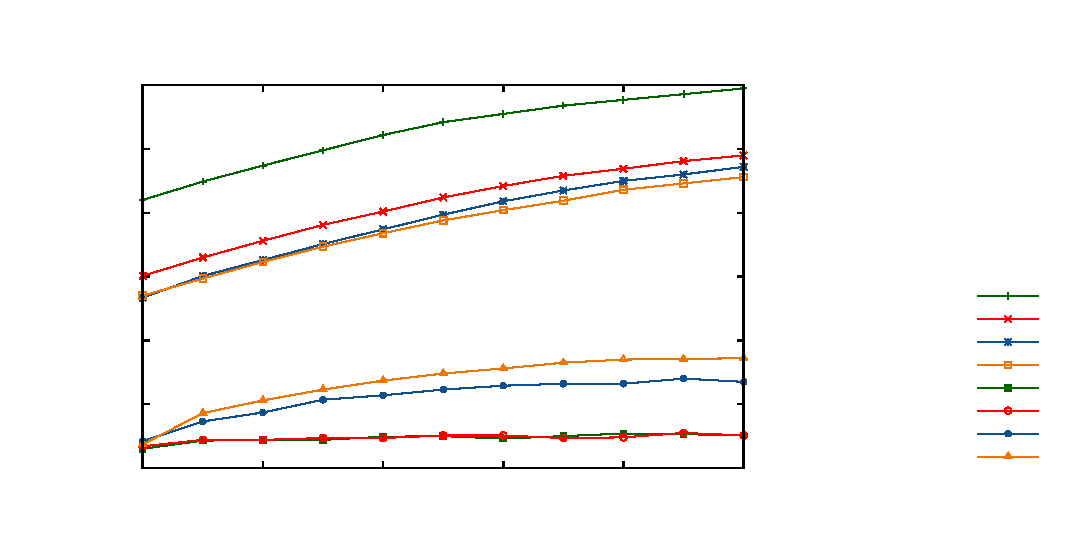
\includegraphics{benchData/bench_output_5000000_10_10_js1}}%
    \gplfronttext
  \end{picture}%
\endgroup
}\end{center}
\caption{Πίνακας και διάγραμμα χρόνομέτρησης της μέτρησης: 5 εκατομμύρια ζεύγη/10 επαναλήψεις/σύστημα 3.}
\label{gpuexample}
\end{figure}

Η μέθοδος παράλληλης επεξεργασίας που εφαρμόζεται στις GPU φέρνει διαφορετικά αποτελέσματα. Κάθε υπολογιστική μονάδα μιας GPU εκτελεί παράλληλα έναν μεγάλο αριθμό αντικειμένων εργασίας τα οποία ανήκουν σε μια ομάδα εργασίας. Η επεξεργασία της κάθε ομάδας εργασίας θεωρείται ότι έχει ολοκληρωθεί μόνο όταν τερματιστεί η επεξεργασία καθενός από τα αντικείμενα εργασίας που της ανήκουν. Αυτό σημαίνει ότι, αν και τα αντικείμενα εργασίας μέσα στην ομάδα μπορούν να ακολουθήσουν πολλά και διαφορετικά μονοπάτια εκτέλεσης με διαφορετικές ταχύτητες, τα εξαγόμενα τους αποθηκεύονται στην μνήμη μόνο όταν τερματίσουν και αυτά με το αργότερο μονοπάτι εκτέλεσης. Στην γενική περίπτωση αυτό σημαίνει ότι οι χρόνοι επεξεργασίας των αλγορίθμων GPU επηρεάζονται λιγότερο από το ποσοστό τεμνόμενων ζευγών, καθώς η ομαδοποίηση των αντικειμένων εργασίας τείνει να εξισώσει τον χρόνο επεξεργασίας ανάμεσα στις περιπτώσεις ύπαρξης και μη ύπαρξης τομής. Η μεταβολή του χρόνου επεξεργασίας είναι μικρότερη και πιο ακανόνιστη σε σχέση με την 
περίπτωση των αλγορίθμων CPU.

Χαρακτηριστικό παράδειγμα της διαφοροποίησης επιδόσεων μεταξύ CPU και GPU είναι η μέτρηση με 5 εκατομμύρια ζεύγη και 10 επαναλήψεις στο σύστημα 3 (Linux), τα αποτελέσματα τις οποίας παρουσιάζονται στο σχήμα \ref{gpuexample}. Σε αυτή, ο συνολικός χρόνος εκτέλεσης (συμπεριλαμβανομένων των χρόνων μεταφορών) των αλγορίθμων σε GPU είναι υποπολλαπλάσιος των αντίστοιχων σε CPU σε κάθε περίπτωση. Στις μη βελτιστοποιημένες μορφές των αλγορίθμων (Plucker0, STP0) οι υλοποιήσεις σε GPU εκτελούνται κατα προσέγγιση στο $1/5$ του χρόνου των αντίστοιχων. Στην βελτιστοποιημένη μορφή 2 η διαφορά ελαττώνεται στο $1/2$. Επίσης, το διάγραμμα χρόνου επεξεργασίας παρέχει μια άμεση σύγκριση της διαφορετικής επιρροής του ποσοστού τεμνόμενων ζευγών ανάμεσα στους αλγορίθμους CPU και GPU.



\subsection{Αποτελεσματικότητα μορφών αλγορίθμων σε CPU και GPU}
\label{chapter:bench_algs}
\noindent Η κατάταξη των αλγορίθμων με βάση την ταχύτητα επεξεργασίας τους διαφέρει ριζικά ανάμεσα στις υλοποιήσεις σε CPU και GPU. Στην πλειοψηφία των περιπτώσεων οι αλγόριθμοι σε CPU κατατάσσονται με βάση την ταχύτητα εκτέλεσης τους, σε φθίνουσα σειρά, ως εξής:

\begin{enumerate*}
\item STP1
\item STP2
\item STP0
\item Plücker1
\item Plücker2
\item Plücker0
\end{enumerate*}

Η σειρά αυτή βρίσκεται σε συμφωνία με τα αποτελέσματα των μετρήσεων της δημοσίευσης \cite{PlatisTheoharis03}. Οι μορφές αλγορίθμου με χρήση μεικτού γινομένου είναι γενικά ταχύτερες από τις αντίστοιχες των συντεταγμένων Plücker. Μεταξύ των διαφορετικών μορφών βελτιστοποίησης αναδεικνύεται ως ταχύτερη η μορφή 1. Όπως αναφέρεται στο \cite{PlatisTheoharis03}, εξετάζοντας την περίπτωση των αλγορίθμων συντεταγμένων Plücker, η μεγαλύτερη πολυπλοκότητα της μορφής 2 την καθιστά αργότερη από την 1. Στις δοκιμές που έγιναν στα πλαίσια της εργασίας αυτής φαίνεται να ισχύει το ίδιο και για τους αλγορίθμους μεικτού γινομένου, με μία εξαίρεση: στις δοκιμές στο σύστημα 3, ιδιαίτερα σε αυτές με υψηλά ποσοστά τεμνόμενων ζευγών, η μορφή 2 μεικτού γινομένου είναι ταχύτερη της 1. Οι σχετικές επιδόσεις των αλγορίθμων CPU στα συστήματα 1 και 3 εμφανίζονται στο σχήμα \ref{effcpuexample}.

\begin{figure}[h!]
\begin{center}
\scalebox{0.9}
{
% GNUPLOT: LaTeX picture with Postscript
\begingroup
  \makeatletter
  \providecommand\color[2][]{%
    \GenericError{(gnuplot) \space\space\space\@spaces}{%
      Package color not loaded in conjunction with
      terminal option `colourtext'%
    }{See the gnuplot documentation for explanation.%
    }{Either use 'blacktext' in gnuplot or load the package
      color.sty in LaTeX.}%
    \renewcommand\color[2][]{}%
  }%
  \providecommand\includegraphics[2][]{%
    \GenericError{(gnuplot) \space\space\space\@spaces}{%
      Package graphicx or graphics not loaded%
    }{See the gnuplot documentation for explanation.%
    }{The gnuplot epslatex terminal needs graphicx.sty or graphics.sty.}%
    \renewcommand\includegraphics[2][]{}%
  }%
  \providecommand\rotatebox[2]{#2}%
  \@ifundefined{ifGPcolor}{%
    \newif\ifGPcolor
    \GPcolorfalse
  }{}%
  \@ifundefined{ifGPblacktext}{%
    \newif\ifGPblacktext
    \GPblacktexttrue
  }{}%
  % define a \g@addto@macro without @ in the name:
  \let\gplgaddtomacro\g@addto@macro
  % define empty templates for all commands taking text:
  \gdef\gplbacktext{}%
  \gdef\gplfronttext{}%
  \makeatother
  \ifGPblacktext
    % no textcolor at all
    \def\colorrgb#1{}%
    \def\colorgray#1{}%
  \else
    % gray or color?
    \ifGPcolor
      \def\colorrgb#1{\color[rgb]{#1}}%
      \def\colorgray#1{\color[gray]{#1}}%
      \expandafter\def\csname LTw\endcsname{\color{white}}%
      \expandafter\def\csname LTb\endcsname{\color{black}}%
      \expandafter\def\csname LTa\endcsname{\color{black}}%
      \expandafter\def\csname LT0\endcsname{\color[rgb]{1,0,0}}%
      \expandafter\def\csname LT1\endcsname{\color[rgb]{0,1,0}}%
      \expandafter\def\csname LT2\endcsname{\color[rgb]{0,0,1}}%
      \expandafter\def\csname LT3\endcsname{\color[rgb]{1,0,1}}%
      \expandafter\def\csname LT4\endcsname{\color[rgb]{0,1,1}}%
      \expandafter\def\csname LT5\endcsname{\color[rgb]{1,1,0}}%
      \expandafter\def\csname LT6\endcsname{\color[rgb]{0,0,0}}%
      \expandafter\def\csname LT7\endcsname{\color[rgb]{1,0.3,0}}%
      \expandafter\def\csname LT8\endcsname{\color[rgb]{0.5,0.5,0.5}}%
    \else
      % gray
      \def\colorrgb#1{\color{black}}%
      \def\colorgray#1{\color[gray]{#1}}%
      \expandafter\def\csname LTw\endcsname{\color{white}}%
      \expandafter\def\csname LTb\endcsname{\color{black}}%
      \expandafter\def\csname LTa\endcsname{\color{black}}%
      \expandafter\def\csname LT0\endcsname{\color{black}}%
      \expandafter\def\csname LT1\endcsname{\color{black}}%
      \expandafter\def\csname LT2\endcsname{\color{black}}%
      \expandafter\def\csname LT3\endcsname{\color{black}}%
      \expandafter\def\csname LT4\endcsname{\color{black}}%
      \expandafter\def\csname LT5\endcsname{\color{black}}%
      \expandafter\def\csname LT6\endcsname{\color{black}}%
      \expandafter\def\csname LT7\endcsname{\color{black}}%
      \expandafter\def\csname LT8\endcsname{\color{black}}%
    \fi
  \fi
  \setlength{\unitlength}{0.0500bp}%
  \begin{picture}(10080.00,5040.00)%
    \gplgaddtomacro\gplbacktext{%
      \csname LTb\endcsname%
      \put(1078,704){\makebox(0,0)[r]{\strut{} 2500}}%
      \put(1078,1229){\makebox(0,0)[r]{\strut{} 3000}}%
      \put(1078,1754){\makebox(0,0)[r]{\strut{} 3500}}%
      \put(1078,2279){\makebox(0,0)[r]{\strut{} 4000}}%
      \put(1078,2804){\makebox(0,0)[r]{\strut{} 4500}}%
      \put(1078,3329){\makebox(0,0)[r]{\strut{} 5000}}%
      \put(1078,3854){\makebox(0,0)[r]{\strut{} 5500}}%
      \put(1078,4379){\makebox(0,0)[r]{\strut{} 6000}}%
      \put(1210,484){\makebox(0,0){\strut{} 0}}%
      \put(2469,484){\makebox(0,0){\strut{} 20}}%
      \put(3729,484){\makebox(0,0){\strut{} 40}}%
      \put(4988,484){\makebox(0,0){\strut{} 60}}%
      \put(6248,484){\makebox(0,0){\strut{} 80}}%
      \put(7507,484){\makebox(0,0){\strut{} 100}}%
      \put(176,2541){\rotatebox{-270}{\makebox(0,0){\strut{}Χρόνος (ms)}}}%
      \put(4358,154){\makebox(0,0){\strut{}Ποσοστό τεμνόμενων ζευγών \%}}%
      \put(4358,4709){\makebox(0,0){\strut{}Χρόνος Επεξεργασίας (Σύστημα 1)}}%
    }%
    \gplgaddtomacro\gplfronttext{%
      \csname LTb\endcsname%
      \put(9091,1914){\makebox(0,0)[r]{\strut{}Plücker 0}}%
      \csname LTb\endcsname%
      \put(9091,1694){\makebox(0,0)[r]{\strut{}Plücker 1}}%
      \csname LTb\endcsname%
      \put(9091,1474){\makebox(0,0)[r]{\strut{}Plücker 2}}%
      \csname LTb\endcsname%
      \put(9091,1254){\makebox(0,0)[r]{\strut{}STP 0}}%
      \csname LTb\endcsname%
      \put(9091,1034){\makebox(0,0)[r]{\strut{}STP 1}}%
      \csname LTb\endcsname%
      \put(9091,814){\makebox(0,0)[r]{\strut{}STP 2}}%
    }%
    \gplbacktext
    \put(0,0){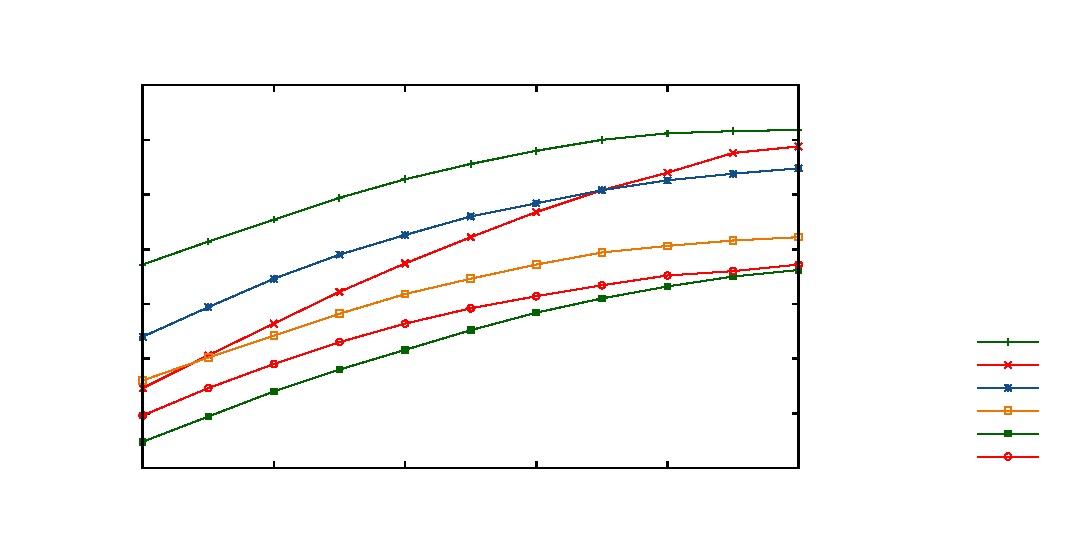
\includegraphics{benchData/cpu_graph.eps}}%
    \gplfronttext
  \end{picture}%
\endgroup

}
\scalebox{0.9}
{
% GNUPLOT: LaTeX picture with Postscript
\begingroup
  \makeatletter
  \providecommand\color[2][]{%
    \GenericError{(gnuplot) \space\space\space\@spaces}{%
      Package color not loaded in conjunction with
      terminal option `colourtext'%
    }{See the gnuplot documentation for explanation.%
    }{Either use 'blacktext' in gnuplot or load the package
      color.sty in LaTeX.}%
    \renewcommand\color[2][]{}%
  }%
  \providecommand\includegraphics[2][]{%
    \GenericError{(gnuplot) \space\space\space\@spaces}{%
      Package graphicx or graphics not loaded%
    }{See the gnuplot documentation for explanation.%
    }{The gnuplot epslatex terminal needs graphicx.sty or graphics.sty.}%
    \renewcommand\includegraphics[2][]{}%
  }%
  \providecommand\rotatebox[2]{#2}%
  \@ifundefined{ifGPcolor}{%
    \newif\ifGPcolor
    \GPcolorfalse
  }{}%
  \@ifundefined{ifGPblacktext}{%
    \newif\ifGPblacktext
    \GPblacktexttrue
  }{}%
  % define a \g@addto@macro without @ in the name:
  \let\gplgaddtomacro\g@addto@macro
  % define empty templates for all commands taking text:
  \gdef\gplbacktext{}%
  \gdef\gplfronttext{}%
  \makeatother
  \ifGPblacktext
    % no textcolor at all
    \def\colorrgb#1{}%
    \def\colorgray#1{}%
  \else
    % gray or color?
    \ifGPcolor
      \def\colorrgb#1{\color[rgb]{#1}}%
      \def\colorgray#1{\color[gray]{#1}}%
      \expandafter\def\csname LTw\endcsname{\color{white}}%
      \expandafter\def\csname LTb\endcsname{\color{black}}%
      \expandafter\def\csname LTa\endcsname{\color{black}}%
      \expandafter\def\csname LT0\endcsname{\color[rgb]{1,0,0}}%
      \expandafter\def\csname LT1\endcsname{\color[rgb]{0,1,0}}%
      \expandafter\def\csname LT2\endcsname{\color[rgb]{0,0,1}}%
      \expandafter\def\csname LT3\endcsname{\color[rgb]{1,0,1}}%
      \expandafter\def\csname LT4\endcsname{\color[rgb]{0,1,1}}%
      \expandafter\def\csname LT5\endcsname{\color[rgb]{1,1,0}}%
      \expandafter\def\csname LT6\endcsname{\color[rgb]{0,0,0}}%
      \expandafter\def\csname LT7\endcsname{\color[rgb]{1,0.3,0}}%
      \expandafter\def\csname LT8\endcsname{\color[rgb]{0.5,0.5,0.5}}%
    \else
      % gray
      \def\colorrgb#1{\color{black}}%
      \def\colorgray#1{\color[gray]{#1}}%
      \expandafter\def\csname LTw\endcsname{\color{white}}%
      \expandafter\def\csname LTb\endcsname{\color{black}}%
      \expandafter\def\csname LTa\endcsname{\color{black}}%
      \expandafter\def\csname LT0\endcsname{\color{black}}%
      \expandafter\def\csname LT1\endcsname{\color{black}}%
      \expandafter\def\csname LT2\endcsname{\color{black}}%
      \expandafter\def\csname LT3\endcsname{\color{black}}%
      \expandafter\def\csname LT4\endcsname{\color{black}}%
      \expandafter\def\csname LT5\endcsname{\color{black}}%
      \expandafter\def\csname LT6\endcsname{\color{black}}%
      \expandafter\def\csname LT7\endcsname{\color{black}}%
      \expandafter\def\csname LT8\endcsname{\color{black}}%
    \fi
  \fi
  \setlength{\unitlength}{0.0500bp}%
  \begin{picture}(10080.00,5040.00)%
    \gplgaddtomacro\gplbacktext{%
      \csname LTb\endcsname%
      \put(1078,704){\makebox(0,0)[r]{\strut{} 2500}}%
      \put(1078,1229){\makebox(0,0)[r]{\strut{} 3000}}%
      \put(1078,1754){\makebox(0,0)[r]{\strut{} 3500}}%
      \put(1078,2279){\makebox(0,0)[r]{\strut{} 4000}}%
      \put(1078,2804){\makebox(0,0)[r]{\strut{} 4500}}%
      \put(1078,3329){\makebox(0,0)[r]{\strut{} 5000}}%
      \put(1078,3854){\makebox(0,0)[r]{\strut{} 5500}}%
      \put(1078,4379){\makebox(0,0)[r]{\strut{} 6000}}%
      \put(1210,484){\makebox(0,0){\strut{} 0}}%
      \put(2469,484){\makebox(0,0){\strut{} 20}}%
      \put(3729,484){\makebox(0,0){\strut{} 40}}%
      \put(4988,484){\makebox(0,0){\strut{} 60}}%
      \put(6248,484){\makebox(0,0){\strut{} 80}}%
      \put(7507,484){\makebox(0,0){\strut{} 100}}%
      \put(176,2541){\rotatebox{-270}{\makebox(0,0){\strut{}Χρόνος (ms)}}}%
      \put(4358,154){\makebox(0,0){\strut{}Ποσοστό τεμνόμενων ζευγών \%}}%
      \put(4358,4709){\makebox(0,0){\strut{}Χρόνος Επεξεργασίας (Σύστημα 3)}}%
    }%
    \gplgaddtomacro\gplfronttext{%
      \csname LTb\endcsname%
      \put(9091,1914){\makebox(0,0)[r]{\strut{}Plücker 0}}%
      \csname LTb\endcsname%
      \put(9091,1694){\makebox(0,0)[r]{\strut{}Plücker 1}}%
      \csname LTb\endcsname%
      \put(9091,1474){\makebox(0,0)[r]{\strut{}Plücker 2}}%
      \csname LTb\endcsname%
      \put(9091,1254){\makebox(0,0)[r]{\strut{}STP 0}}%
      \csname LTb\endcsname%
      \put(9091,1034){\makebox(0,0)[r]{\strut{}STP 1}}%
      \csname LTb\endcsname%
      \put(9091,814){\makebox(0,0)[r]{\strut{}STP 2}}%
    }%
    \gplbacktext
    \put(0,0){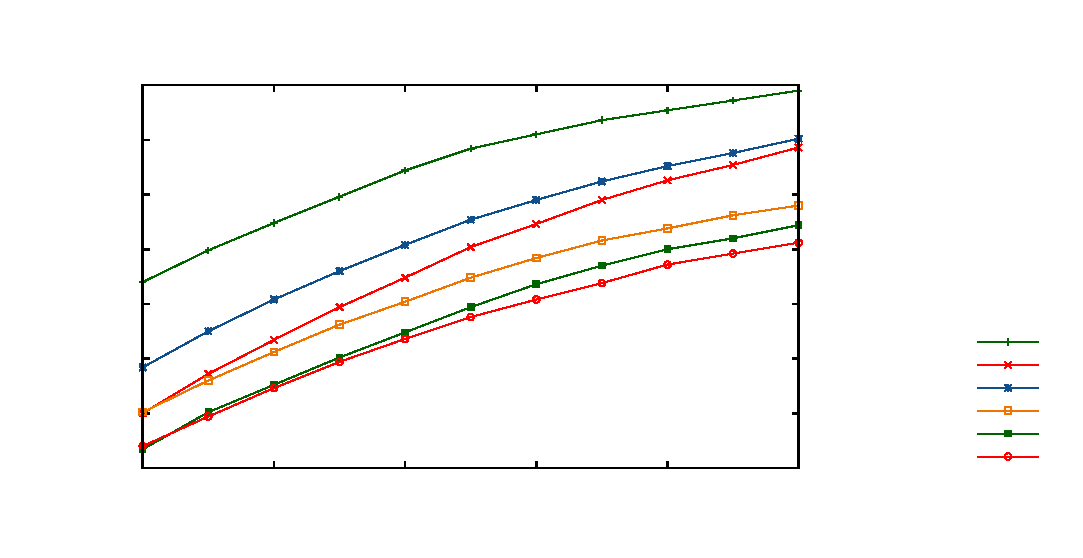
\includegraphics{benchData/cpu_graph_3.eps}}%
    \gplfronttext
  \end{picture}%
\endgroup

}
\end{center}
\caption{Σύγκριση της σχετικής απόδοσης των αλγορίθμων CPU στα συστήματα 1 και 3. Βασίζεται στην δοκιμή:2,5 εκατομμύρια ζεύγη/10 επαναλήψεις. Και στα στα συστήματα χρησιμοποιείται η υλοποίηση σε Linux.}
\label{effcpuexample}
\end{figure}

Οι υλοποιήσεις σε GPU εμφανίζουν εντελώς διαφορετική εικόνα. Οι μη βελτιστοποιημένες μορφές 0 είναι ταχύτερες σε όλες τις περιπτώσεις από τις 1 και 2, με την STP0 να είναι ελαφρώς ταχύτερη της Plücker0. Αυτό οφείλεται στο γεγονός ότι η απλή ροή ελέγχου που ακολουθεί η μορφή 0 προσαρμόζεται πολύ καλύτερα στον τρόπο λειτουργίας της GPU απ' ότι αυτές των μορφών 1 και 2.

Η αρχιτεκτονική των σύγχρονων GPU, όπως έχει αναφερθεί, έχει αναπτυχθεί με γνώμονα την βελτιστοποίηση της διεκπεραιωτικής τους ικανότητας κατά την επεξεργασία μεγάλων ποσοτήτων δεδομένων κινητής υποδιαστολής. Η έμφαση στην ταχύτητα της επεξεργασίας έχει ως αποτέλεσμα οι GPU να περιλαμβάνουν πολύ απλούστερες μονάδες ελέγχου σε σχέση με τις CPU. Κατά συνέπεια, οι εντολές διακλάδωσης έχουν σημαντικά μεγαλύτερο χρονικό κόστος από τις εντολές υπολογισμού. Αυτό σημαίνει πως η πολυπλοκότητα των δομών ελέγχου και επανάληψης του κώδικα που εκτελείται στην GPU έχει άμεση επίδραση στις επιδόσεις του. Μια μικρή αύξηση της πολυπλοκότητας αυτής μπορεί να μειώσει δραστικά την ταχύτητα εκτέλεσης. Οι κατασκευαστές GPU προτείνουν γενικά την χρήση όσο το δυνατόν απλούστερων δομών ελέγχου στον προγραμματισμό των συσκευών τους \cite{ATIOpenCL}.

Το σχήμα \ref{effgpuexample} παρουσιάζει τις σχετικές επιδόσεις των αλγορίθμων GPU στην δοκιμή με 2,5 εκατομμύρια ζεύγη και 10 επαναλήψεις στο σύστημα 1.

\begin{figure}[h!]
\begin{center}
\scalebox{0.9}
{
% GNUPLOT: LaTeX picture with Postscript
\begingroup
  \makeatletter
  \providecommand\color[2][]{%
    \GenericError{(gnuplot) \space\space\space\@spaces}{%
      Package color not loaded in conjunction with
      terminal option `colourtext'%
    }{See the gnuplot documentation for explanation.%
    }{Either use 'blacktext' in gnuplot or load the package
      color.sty in LaTeX.}%
    \renewcommand\color[2][]{}%
  }%
  \providecommand\includegraphics[2][]{%
    \GenericError{(gnuplot) \space\space\space\@spaces}{%
      Package graphicx or graphics not loaded%
    }{See the gnuplot documentation for explanation.%
    }{The gnuplot epslatex terminal needs graphicx.sty or graphics.sty.}%
    \renewcommand\includegraphics[2][]{}%
  }%
  \providecommand\rotatebox[2]{#2}%
  \@ifundefined{ifGPcolor}{%
    \newif\ifGPcolor
    \GPcolorfalse
  }{}%
  \@ifundefined{ifGPblacktext}{%
    \newif\ifGPblacktext
    \GPblacktexttrue
  }{}%
  % define a \g@addto@macro without @ in the name:
  \let\gplgaddtomacro\g@addto@macro
  % define empty templates for all commands taking text:
  \gdef\gplbacktext{}%
  \gdef\gplfronttext{}%
  \makeatother
  \ifGPblacktext
    % no textcolor at all
    \def\colorrgb#1{}%
    \def\colorgray#1{}%
  \else
    % gray or color?
    \ifGPcolor
      \def\colorrgb#1{\color[rgb]{#1}}%
      \def\colorgray#1{\color[gray]{#1}}%
      \expandafter\def\csname LTw\endcsname{\color{white}}%
      \expandafter\def\csname LTb\endcsname{\color{black}}%
      \expandafter\def\csname LTa\endcsname{\color{black}}%
      \expandafter\def\csname LT0\endcsname{\color[rgb]{1,0,0}}%
      \expandafter\def\csname LT1\endcsname{\color[rgb]{0,1,0}}%
      \expandafter\def\csname LT2\endcsname{\color[rgb]{0,0,1}}%
      \expandafter\def\csname LT3\endcsname{\color[rgb]{1,0,1}}%
      \expandafter\def\csname LT4\endcsname{\color[rgb]{0,1,1}}%
      \expandafter\def\csname LT5\endcsname{\color[rgb]{1,1,0}}%
      \expandafter\def\csname LT6\endcsname{\color[rgb]{0,0,0}}%
      \expandafter\def\csname LT7\endcsname{\color[rgb]{1,0.3,0}}%
      \expandafter\def\csname LT8\endcsname{\color[rgb]{0.5,0.5,0.5}}%
    \else
      % gray
      \def\colorrgb#1{\color{black}}%
      \def\colorgray#1{\color[gray]{#1}}%
      \expandafter\def\csname LTw\endcsname{\color{white}}%
      \expandafter\def\csname LTb\endcsname{\color{black}}%
      \expandafter\def\csname LTa\endcsname{\color{black}}%
      \expandafter\def\csname LT0\endcsname{\color{black}}%
      \expandafter\def\csname LT1\endcsname{\color{black}}%
      \expandafter\def\csname LT2\endcsname{\color{black}}%
      \expandafter\def\csname LT3\endcsname{\color{black}}%
      \expandafter\def\csname LT4\endcsname{\color{black}}%
      \expandafter\def\csname LT5\endcsname{\color{black}}%
      \expandafter\def\csname LT6\endcsname{\color{black}}%
      \expandafter\def\csname LT7\endcsname{\color{black}}%
      \expandafter\def\csname LT8\endcsname{\color{black}}%
    \fi
  \fi
  \setlength{\unitlength}{0.0500bp}%
  \begin{picture}(10080.00,5040.00)%
    \gplgaddtomacro\gplbacktext{%
      \csname LTb\endcsname%
      \put(946,704){\makebox(0,0)[r]{\strut{} 200}}%
      \put(946,1072){\makebox(0,0)[r]{\strut{} 250}}%
      \put(946,1439){\makebox(0,0)[r]{\strut{} 300}}%
      \put(946,1807){\makebox(0,0)[r]{\strut{} 350}}%
      \put(946,2174){\makebox(0,0)[r]{\strut{} 400}}%
      \put(946,2542){\makebox(0,0)[r]{\strut{} 450}}%
      \put(946,2909){\makebox(0,0)[r]{\strut{} 500}}%
      \put(946,3277){\makebox(0,0)[r]{\strut{} 550}}%
      \put(946,3644){\makebox(0,0)[r]{\strut{} 600}}%
      \put(946,4012){\makebox(0,0)[r]{\strut{} 650}}%
      \put(946,4379){\makebox(0,0)[r]{\strut{} 700}}%
      \put(1078,484){\makebox(0,0){\strut{} 0}}%
      \put(2364,484){\makebox(0,0){\strut{} 20}}%
      \put(3650,484){\makebox(0,0){\strut{} 40}}%
      \put(4935,484){\makebox(0,0){\strut{} 60}}%
      \put(6221,484){\makebox(0,0){\strut{} 80}}%
      \put(7507,484){\makebox(0,0){\strut{} 100}}%
      \put(176,2541){\rotatebox{-270}{\makebox(0,0){\strut{}Χρόνος (ms)}}}%
      \put(4292,154){\makebox(0,0){\strut{}Ποσοστό τεμνόμενων ζευγών \%}}%
      \put(4292,4709){\makebox(0,0){\strut{}Χρόνος Επεξεργασίας}}%
    }%
    \gplgaddtomacro\gplfronttext{%
      \csname LTb\endcsname%
      \put(9091,1474){\makebox(0,0)[r]{\strut{}Plücker 0}}%
      \csname LTb\endcsname%
      \put(9091,1254){\makebox(0,0)[r]{\strut{}STP 0}}%
      \csname LTb\endcsname%
      \put(9091,1034){\makebox(0,0)[r]{\strut{}STP 1}}%
      \csname LTb\endcsname%
      \put(9091,814){\makebox(0,0)[r]{\strut{}STP 2}}%
    }%
    \gplbacktext
    \put(0,0){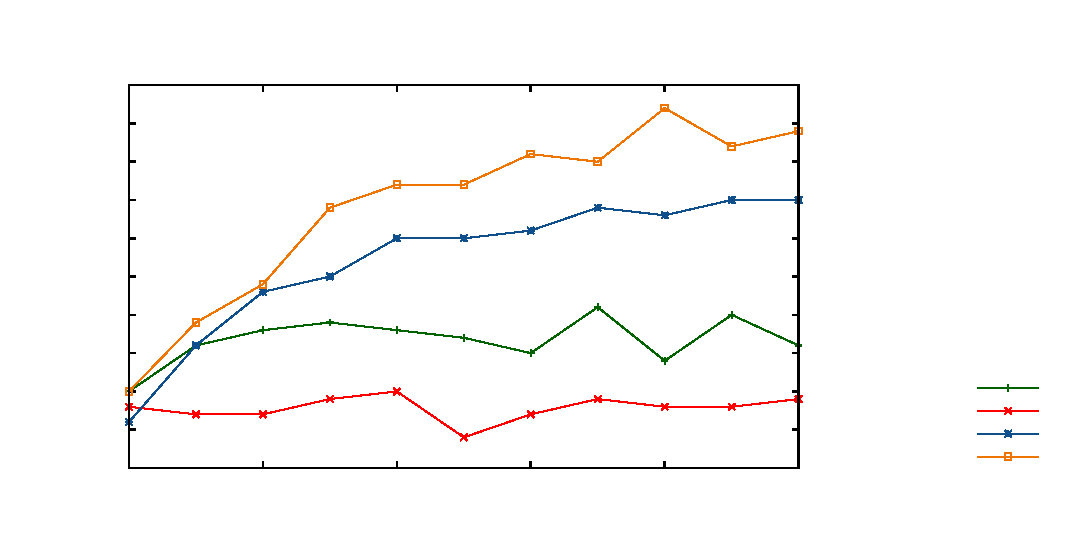
\includegraphics{benchData/gpu_graph.eps}}%
    \gplfronttext
  \end{picture}%
\endgroup

}
\end{center}
\caption{Σύγκριση της σχετικής απόδοσης των αλγορίθμων GPU στην δοκιμή:2,5 εκατομμύρια ζεύγη/10 επαναλήψεις/σύστημα 3.}
\label{effgpuexample}
\end{figure}

\subsection{Επίδραση των ρυθμίσεων δοκιμών στα αποτελέσματα}
\noindent Δύο παράγοντες των ρυθμίσεων δοκιμών παρουσιάζουν σημαντική επιρροή στα αποτελέσματα των μετρήσεων: ο συνολικός αριθμός ελέγχων τομής που εκτελούνται (δηλαδή η διαφορά μεταξύ των δύο σειρών δοκιμών) και η κατανομή των ελέγχων αυτών σε διαφορετικό αριθμό επαναλήψεων.

Η επίδραση του συνολικού αριθμού ελέγχων στις επιδόσεις ερμηνεύεται εύκολα. Στην περίπτωση των αλγορίθμων CPU η αύξηση του χρόνου επεξεργασίας είναι πρακτικά ανάλογη με αυτήν του αριθμού ελέγχων. Αυτό αντικατοπτρίζεται στο γεγονός ότι οι χρόνοι ενός αλγορίθμου CPU στην σειρά δοκιμών 2 είναι κατά προσέγγιση διπλάσιοι από αυτούς στην σειρά 1. Η αναλογία αυτή ισχύει για όλες τις μορφές αλγορίθμων CPU σε όλες τις πιθανές ρυθμίσεις. Στους αλγορίθμους GPU η εικόνα είναι παρόμοια, με τους χρόνους της σειράς δοκιμών 2 να προσεγγίζουν το διπλάσιο των χρόνων της σειράς 1, με κάποιες μικρές αποκλίσεις. Η μόνη σημαντική διαφορά είναι ότι οι αποκλίσεις  αυτές είναι σε κάποιες περιπτώσεις αρνητικές, δηλαδή οι χρόνοι της σειράς 2 είναι μικρότεροι από το διπλάσιο αυτών της σειράς 1.

Ο αριθμός των επαναλήψεων που χρησιμοποιούνται σε κάθε δοκιμή επηρεάζει αρνητικά τις επιδόσεις των αλγορίθμων GPU. Σε όλες τις περιπτώσεις, η αύξηση των επαναλήψεων μεταξύ των δοκιμών φαίνεται να έχει αρνητική επίδραση στις επιδόσεις των αλγορίθμων αυτών, αν και ο συνολικός αριθμός των ελέγχων τομής που εκτελείται παραμένει αμετάβλητος. Αυτό οφείλεται στο γεγονός ότι η έναρξη και η λήξη της εκτέλεσης ενός πυρήνα υπολογισμού στην GPU περιέχουν κάποιο λανθάνοντα χρόνο προετοιμασίας και εκτέλεσης βοηθητικών διαδικασιών \cite{ATIOpenCL}. Καθώς η κάθε επανάληψη περιέχει μια εκτέλεση πυρήνα, οι λανθάνοντες χρόνοι αυτοί αποτυπώνονται αθροιστικά στον χρόνο επεξεργασίας. Όταν ο αριθμός των εκτελέσεων αυξάνεται, η αθροιστική αυτή επίδραση  γίνεται μεγαλύτερη. Στα πλαίσια των μετρήσεων που παρουσιάζονται η αύξηση του χρόνου εκτέλεσης λόγω των επαναλήψεων δεν είναι ιδιαίτερα μεγάλη. Σε μετρήσεις με μεγαλύτερο αριθμό επαναλήψεων (της τάξης των 10 και 100 χιλιάδων), που έγιναν κατά την ανάπτυξη της υλοποίησης σε GPU, 
παρατηρήθηκε σημαντική μείωση επιδόσεων. Τίποτα από τα παραπάνω δεν ισχύει στην περίπτωση των αλγορίθμων CPU, όπου όλες οι διαρρυθμίσεις που έχουν τον ίδιο συνολικό αριθμό ελέγχων τομής παρουσιάζουν πρακτικά ίδιους χρόνους επεξεργασίας.

\subsection{Σύγκριση επιδόσεων μεταξύ λειτουργικών συστημάτων}
\noindent Οι επιδόσεις των δύο εκδόσεων της υλοποίησης της εργασίας, που προορίζονται για τα λειτουργικά συστήματα Linux και Windows 7, συγκρίθηκαν στο σύστημα δοκιμών 3. Ενώ και στις δύο περιπτώσεις εκτελείται ο ίδιος κώδικας στο ίδιο υλικό, παρατηρούνται αξιοσημείωτες διαφορές στις επιδόσεις των αλγορίθμων GPU μεταξύ των δύο λειτουργικών συστημάτων.

Στο σχήμα \ref{gpuoscomp} παρουσιάζονται οι χρόνοι επεξεργασίας των αλγορίθμων GPU στην δοκιμή με 5 εκατομμύρια ζεύγη και 10 επαναλήψεις. Όλοι οι αλγόριθμοι είναι σημαντικά ταχύτεροι στην έκδοση για Windows. Η διαφορά αυτή είναι σχετικά μικρή για τις μη βελτιστοποιημένες μορφές 0 των αλγορίθμων αλλά πολλαπλασιάζεται στις μορφές STP1 και STP2. Επίσης, η απόκριση των αλγορίθμων στο ποσοστό τεμνόμενων ζευγών είναι εντελώς διαφορετική. Οι χρόνοι επεξεργασίας των αλγορίθμων της έκδοσης για Windows μεταβάλλονται ελάχιστα σε σχέση με το ποσοστό τεμνόμενων ζευγών, δίνοντας ένα σχεδόν επίπεδο γράφημα. Οι διαφορές στην απόδοση μεταξύ των τριών μορφών του αλγορίθμου σε αυτή την έκδοση είναι σημαντικά μικρότερες από αυτές σε όλες τις εκδόσεις για Linux.

Οι επιδόσεις των αλγορίθμων CPU είναι πρακτικά ίδιες μεταξύ των δύο λειτουργικών συστημάτων. 

\begin{figure}[h!]
\begin{center}
\scalebox{1.05}
{
% GNUPLOT: LaTeX picture with Postscript
\begingroup
  \makeatletter
  \providecommand\color[2][]{%
    \GenericError{(gnuplot) \space\space\space\@spaces}{%
      Package color not loaded in conjunction with
      terminal option `colourtext'%
    }{See the gnuplot documentation for explanation.%
    }{Either use 'blacktext' in gnuplot or load the package
      color.sty in LaTeX.}%
    \renewcommand\color[2][]{}%
  }%
  \providecommand\includegraphics[2][]{%
    \GenericError{(gnuplot) \space\space\space\@spaces}{%
      Package graphicx or graphics not loaded%
    }{See the gnuplot documentation for explanation.%
    }{The gnuplot epslatex terminal needs graphicx.sty or graphics.sty.}%
    \renewcommand\includegraphics[2][]{}%
  }%
  \providecommand\rotatebox[2]{#2}%
  \@ifundefined{ifGPcolor}{%
    \newif\ifGPcolor
    \GPcolorfalse
  }{}%
  \@ifundefined{ifGPblacktext}{%
    \newif\ifGPblacktext
    \GPblacktexttrue
  }{}%
  % define a \g@addto@macro without @ in the name:
  \let\gplgaddtomacro\g@addto@macro
  % define empty templates for all commands taking text:
  \gdef\gplbacktext{}%
  \gdef\gplfronttext{}%
  \makeatother
  \ifGPblacktext
    % no textcolor at all
    \def\colorrgb#1{}%
    \def\colorgray#1{}%
  \else
    % gray or color?
    \ifGPcolor
      \def\colorrgb#1{\color[rgb]{#1}}%
      \def\colorgray#1{\color[gray]{#1}}%
      \expandafter\def\csname LTw\endcsname{\color{white}}%
      \expandafter\def\csname LTb\endcsname{\color{black}}%
      \expandafter\def\csname LTa\endcsname{\color{black}}%
      \expandafter\def\csname LT0\endcsname{\color[rgb]{1,0,0}}%
      \expandafter\def\csname LT1\endcsname{\color[rgb]{0,1,0}}%
      \expandafter\def\csname LT2\endcsname{\color[rgb]{0,0,1}}%
      \expandafter\def\csname LT3\endcsname{\color[rgb]{1,0,1}}%
      \expandafter\def\csname LT4\endcsname{\color[rgb]{0,1,1}}%
      \expandafter\def\csname LT5\endcsname{\color[rgb]{1,1,0}}%
      \expandafter\def\csname LT6\endcsname{\color[rgb]{0,0,0}}%
      \expandafter\def\csname LT7\endcsname{\color[rgb]{1,0.3,0}}%
      \expandafter\def\csname LT8\endcsname{\color[rgb]{0.5,0.5,0.5}}%
    \else
      % gray
      \def\colorrgb#1{\color{black}}%
      \def\colorgray#1{\color[gray]{#1}}%
      \expandafter\def\csname LTw\endcsname{\color{white}}%
      \expandafter\def\csname LTb\endcsname{\color{black}}%
      \expandafter\def\csname LTa\endcsname{\color{black}}%
      \expandafter\def\csname LT0\endcsname{\color{black}}%
      \expandafter\def\csname LT1\endcsname{\color{black}}%
      \expandafter\def\csname LT2\endcsname{\color{black}}%
      \expandafter\def\csname LT3\endcsname{\color{black}}%
      \expandafter\def\csname LT4\endcsname{\color{black}}%
      \expandafter\def\csname LT5\endcsname{\color{black}}%
      \expandafter\def\csname LT6\endcsname{\color{black}}%
      \expandafter\def\csname LT7\endcsname{\color{black}}%
      \expandafter\def\csname LT8\endcsname{\color{black}}%
    \fi
  \fi
  \setlength{\unitlength}{0.0500bp}%
  \begin{picture}(10080.00,5040.00)%
    \gplgaddtomacro\gplbacktext{%
      \csname LTb\endcsname%
      \put(1078,704){\makebox(0,0)[r]{\strut{} 200}}%
      \put(1078,1163){\makebox(0,0)[r]{\strut{} 400}}%
      \put(1078,1623){\makebox(0,0)[r]{\strut{} 600}}%
      \put(1078,2082){\makebox(0,0)[r]{\strut{} 800}}%
      \put(1078,2542){\makebox(0,0)[r]{\strut{} 1000}}%
      \put(1078,3001){\makebox(0,0)[r]{\strut{} 1200}}%
      \put(1078,3460){\makebox(0,0)[r]{\strut{} 1400}}%
      \put(1078,3920){\makebox(0,0)[r]{\strut{} 1600}}%
      \put(1078,4379){\makebox(0,0)[r]{\strut{} 1800}}%
      \put(1210,484){\makebox(0,0){\strut{} 0}}%
      \put(2258,484){\makebox(0,0){\strut{} 20}}%
      \put(3306,484){\makebox(0,0){\strut{} 40}}%
      \put(4355,484){\makebox(0,0){\strut{} 60}}%
      \put(5403,484){\makebox(0,0){\strut{} 80}}%
      \put(6451,484){\makebox(0,0){\strut{} 100}}%
      \put(176,2541){\rotatebox{-270}{\makebox(0,0){\strut{}Χρόνος (ms)}}}%
      \put(3830,154){\makebox(0,0){\strut{}Ποσοστό τεμνόμενων ζευγών \%}}%
      \put(3830,4709){\makebox(0,0){\strut{}Χρόνος Επεξεργασίας}}%
    }%
    \gplgaddtomacro\gplfronttext{%
      \csname LTb\endcsname%
      \put(9091,2354){\makebox(0,0)[r]{\strut{}Plücker 0 Linux}}%
      \csname LTb\endcsname%
      \put(9091,2134){\makebox(0,0)[r]{\strut{}STP 0 Linux}}%
      \csname LTb\endcsname%
      \put(9091,1914){\makebox(0,0)[r]{\strut{}STP 1 Linux}}%
      \csname LTb\endcsname%
      \put(9091,1694){\makebox(0,0)[r]{\strut{}STP 2 Linux}}%
      \csname LTb\endcsname%
      \put(9091,1474){\makebox(0,0)[r]{\strut{}Plücker 0 Windows}}%
      \csname LTb\endcsname%
      \put(9091,1254){\makebox(0,0)[r]{\strut{}STP 0 Windows}}%
      \csname LTb\endcsname%
      \put(9091,1034){\makebox(0,0)[r]{\strut{}STP 1 Windows}}%
      \csname LTb\endcsname%
      \put(9091,814){\makebox(0,0)[r]{\strut{}STP 2 Windows}}%
    }%
    \gplbacktext
    \put(0,0){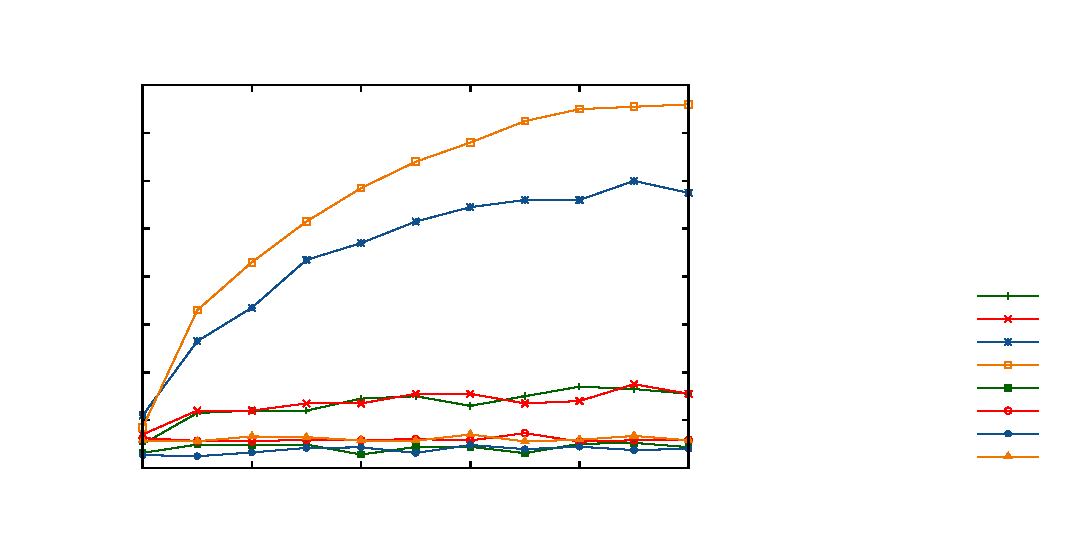
\includegraphics{benchData/linwin}}%
    \gplfronttext
  \end{picture}%
\endgroup

}
\end{center}
\caption{Χρόνοι επεξεργασίας των αλγορίθμων GPU σε Linux και Windows στην δοκιμή 5 εκατομμύρια ζεύγη/10 επαναλήψεις/σύστημα 3.}
\label{gpuoscomp}
\end{figure}

\UndefineShortVerb{\!}